\subsection{Gimlet}
\vspace{-7.4mm}
\hspace{28mm}
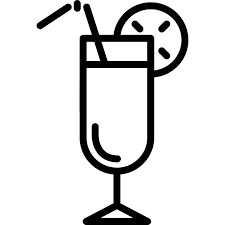
\includegraphics[scale=.07]{cocktail_glass_tall.png}

\includegraphics[scale=.12]{capital_a.png}
\vspace{2.5mm}
\begin{itembox}[l]{\boldmath $\reci$}
\begin{itemize}
\setlength{\parskip}{0cm}
\setlength{\itemsep}{0cm}
\item \gin 45ml
\item \limj 15ml
\item \gumsyrup 1--3tsp
\end{itemize}
\vspace{-4mm}
Made by \shake
\end{itembox}
Turns to Vodka Gimlet by using \vodka instead of \gin
\hspace{-1mm}.
Turns to Gimlet highball by adding \soda
\hspace{-1mm}.
Turns to Nobunaga by using \gs instead of \gumsyrup
\hspace{-1mm}.
